
% 论文正文,章节请根据自己需求进行修改

% 引言,根据自身论文,修改引言的Tex文件
% 引言

\chapter{引~~~~言}
本文主要研究了

\textcolor{blue}{生僻字:垚瑄。}若这行无法看到全部内容,则表示默认\textbackslash{}songti命令不支持生僻字。

\textcolor{blue}{\mystsong{生僻字:垚瑄。}}此行一般可以看到内容,使用方正宋体\textbackslash{}mystsongti命令。

注意到这两种字体存在细微差异,因此一定要注意尽量仅在需要的使用\textbackslash{}mystsongti,并且务必使用大括号全部括起来,如\{\textbackslash{}mystsongti\{生僻字:垚瑄\}\}。

\textcolor{blue}{撰写引言部分,阅后删除}

% 章节模板,成文后将其注释掉即可
% 样例章节
% 章和引用示例-------------------------------------------------------------------------------------

\chapter{一级题目}

\section{二级题目}

正文······\cite{GB/T16159—1996} % 引用示例

\subsection{三级题目}

正文······\cite{Sobieski}。

图、表、公式等非正文文本的内容,应用\textbackslash{}label进行标注,然后用\textbackslash{}ref命令在正文中引用,如图\ref{样式1},表\ref{物流的概念和范围},公式\ref{eqexample}等。正文中一般不应该出现手工输入的编号。
% 章和引用示例-------------------------------------------------------------------------------------

% 图示例----------------------------------------------------------------------------------------
\section{\textcolor{blue}{\underline{\underline{图-示例}}}}

\textcolor{blue}{图的位置:(1)图居中排列。
(2)图与上文之间应留一空行。
(3)图中若有附注,一律用阿拉伯数字按顺序编排,如图\ref{样式1},附注在图的下方。
}

\begin{figure}[htbp]
  \vspace{1mm} % 调整图片与上文的垂直距离
  \centering
  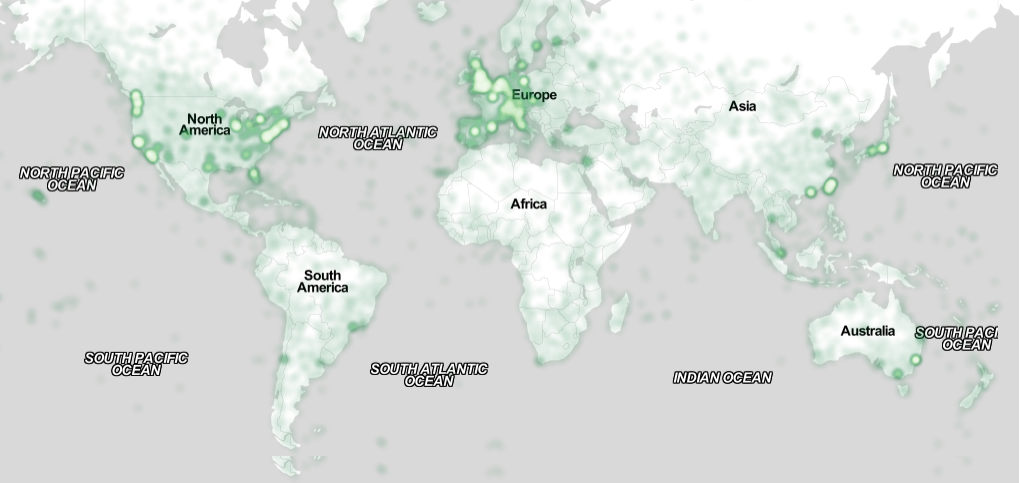
\includegraphics[width=0.8\textwidth]{Images/map.png} % height 可以设置图片的高度, width 可以设置图片的宽度
  \caption{样式1}\label{样式1} % label 用来在文中索引
  \vspace{-6mm} % 调整图片与下文的垂直距离
\end{figure}

下文······
% 图示例----------------------------------------------------------------------------------------

% 公式示例---------------------------------------------------------------------------------------
\section{\textcolor{blue}{\underline{\underline{公式-示例}}}}

\textcolor{blue}{公式标注应于该公式所在行的最右侧。对于较长的公式只可在符号处(+、-、*、/、$\leqslant$ $\geqslant$ 等)转行。在文中引用公式时,在标号前加“式”,如式\ref{eqexample}。}

% 公式上下不要空行,置于同一个段落下即可,否则上下距离会出现高度不一致的问题

\begin{equation}
    LRI=1\ ∕\ \sqrt{ 1 + {\left(\frac{{\mu}_{R}}{{\mu}_{s}}\right)^{2}}{\left(\frac{{\delta}_{R}}{{\delta}_{s}}\right)^{2}} }
    \label{eqexample}
\end{equation}
% 公式示例---------------------------------------------------------------------------------------

% 表示例----------------------------------------------------------------------------------------
\section{\textcolor{blue}{\underline{\underline{表-示例}}}}

\textcolor{blue}{{自动生成LaTeX表工具: \url{https://www.tablesgenerator.com/}}}。见表\ref{物流的概念和范围}和表\ref{统计表}。

\begin{table}[htbp]
  \linespread{1.5}
  \zihao{5}
  \songti
  \centering
  \caption{物流的概念和范围}\label{物流的概念和范围}
  \begin{tabular}{|l|l|}
  \hline
  \multicolumn{1}{|c|}{本 质} & \multicolumn{1}{c|}{过  程}  \\ \hline
  途径或方法                     & 规划、实施、控制                   \\ \hline
  目标                        & 效率、成本效益                    \\ \hline
  活动或作业                     & 流动与储存                      \\ \hline
  处理对象                      & 原材料、在制品、产成品、相关信息           \\ \hline
  范围                        & 从原点(供应商)到终点(最终顾客)          \\ \hline
  目的或目标                     & 适应顾客的需求(产品、功能、数量、质量、时间、价格) \\ \hline
  \end{tabular}
\end{table}

% \begin{table}[htbp]
%   \linespread{1.5}
%   \zihao{5}
%   \songti
%   \centering
%   \caption{统计表}\label{统计表}
%   \begin{tabular}{|l|l|l|l|l|}
%   \hline
%   产品  & 产量    & 销量    & 产值   & 比重    \\ \hline
%   手机  & 11000 & 10000 & 500  & 50\%  \\ \hline
%   电视机 & 5500  & 5000  & 220  & 22\%  \\ \hline
%   计算机 & 1100  & 1000  & 280  & 28\%  \\ \hline
%   合计  & 17600 & 16000 & 1000 & 100\% \\ \hline
%   \end{tabular}
% \end{table}

\begin{table}[htbp]
  \linespread{1.5}
  \zihao{5}
  \songti
  \centering
  \caption{统计表}\label{统计表}
  % Please add the following required packages to your document preamble:
  % \usepackage{multirow}
  \begin{tabular}{|l|l|l|l|l|}
  \hline
  年度                    & 产品  & 产量    & 销量    & 产值  \\ \hline
  \multirow{2}{*}{2004} & 手机  & 11000 & 10000 & 500 \\ \cline{2-5} 
                      & 计算机 & 1100  & 1000  & 280 \\ \hline
  \multirow{2}{*}{2005} & 手机  & 16000 & 13000 & 550 \\ \cline{2-5} 
                      & 计算机 & 2100  & 1500  & 320 \\ \hline
  \end{tabular}
\end{table}
% 表示例----------------------------------------------------------------------------------------

% 伪代码示例------------------------------------------------------------------------------------

\section{\textcolor{blue}{\underline{\underline{伪代码-示例}}}}

\textcolor{blue}{修改 algorithmic 之间的代码就可以实现论文伪代码,已经考虑了伪代码跨页问题,如算法\ref{algoexample}。}
\begin{breakablealgorithm}
        \caption{Calculate $y = x^n$}
        \label{algoexample}
        \begin{algorithmic}[1] %每行显示行号
            \Require $n \geq 0 \vee x \neq 0$ 
            \Ensure  $y = x^n$
            \State $y \gets 1$
            \If{$n < 0$}
            \State $ X \gets 1 / x$
            \State $N \gets -n$
            \Else
            \State $X \gets x$
            \State $N \gets n$
            \EndIf
            \While{ $N \neq 0$ }
            \If{ $N$ is even }
            \State $X \gets x \times x$
            \State $N \gets N / 2$
            \Else[$N$ is odd]
            \State $y \gets y \times X$
            \State $N \gets N - 1$
            \EndIf
            \EndWhile
     \end{algorithmic}
    \end{breakablealgorithm}
% 伪代码示例------------------------------------------------------------------------------------

% 代码块示例------------------------------------------------------------------------------------
\section{\textcolor{blue}{\underline{\underline{代码块-示例}}}}
\textcolor{blue}{只写了 C++, Python, Java 三种语言的格式}

% C++ 代码引入 + 文件引入
\lstinputlisting[
style = C++,
caption = {test.cpp},
label = {test.cpp}
]{./papperCode/test.cpp}

% Java 代码引入 + 行内引入
\begin{lstlisting}[
style = Java,
caption = {test.jar},
label = {test.jar}
]
public class HelloWorld {
    public static void main(String[] args){
        System.out.println("Hello World!");
    }
}
\end{lstlisting}

% Python 代码引入 + 文件引入
\lstinputlisting[
style = Python,
caption = {test.py},
label = {test.py}
]{./papperCode/test.py}
% 代码块示例------------------------------------------------------------------------------------

% 在此插入更多章节
% 第一章
% 根据自身论文修改

\chapter{相关工作}
人工智能算法是时代的热点,在国内外都有许多学者进行研究。
\section{国内研究现状}
\subsection{机器学习}
\subsection{深度学习}

\section{国外研究现状}
\subsection{机器学习}
\subsection{深度学习}

% 结论:根据自身论文,修改结论的Tex文件
%  结论

\unnumchapter{结~~~~论}
\renewcommand{\thechapter}{结论}
\ctexset{
  section/number = \arabic{section}
}

% 结论部分尽量不使用 \subsection 二级标题,只使用 \section 一级标题

% 这里插入一个参考文献,仅作参考
本文结论……。\cite{李成智2004飞行之梦}

\textcolor{blue}{结论作为毕业设计(论文)正文的最后部分单独排写,但不加章号。结论是对整个论文主要结果的总结。在结论中应明确指出本研究的创新点,对其应用前景和社会、经济价值等加以预测和评价,并指出今后进一步在本研究方向进行研究工作的展望与设想。结论部分的撰写应简明扼要,突出创新性。阅后删除此段。}

\textcolor{blue}{结论正文样式与文章正文相同:宋体、小四;行距:22 磅;间距段前段后均为 0 行。阅后删除此段。}

% 参考文献范例章节,成文后应删除本章节
% 参考文献


% 参考文献开始
\unnumchapter{参考文献}
\renewcommand{\thechapter}{参考文献}

% 设置参考文献字号为 5 号
\renewcommand*{\bibfont}{\zihao{5}}
% 设置参考文献各个项目之间的垂直距离为 0
\setlength{\bibitemsep}{0ex}
\setlength{\bibnamesep}{0ex}
\setlength{\bibinitsep}{0ex}
% 设置单倍行距
\renewcommand{\baselinestretch}{1.2}
% 设置参考文献顺序标签 `[1]` 与文献内容 `作者. 文献标题...` 的间距
\setlength{\biblabelsep}{0.5mm}
% 设置参考文献后文缩进为 0(与 Word 模板保持一致)
\renewcommand{\itemcmd}{
  \addvspace{\bibitemsep} % 恢复 \bibitemsep 的作用
  \mkgbnumlabel{\printfield{labelnumber}}
  \hspace{\biblabelsep}}
% 删除默认的「参考文献 / Reference」标题,使用上面定义的 section 标题

\textcolor{blue}{参考文献书写规范}

\textcolor{blue}{参考国家标准《信息与文献参考文献著录规则》【GB/T 7714—2015】,参考文献书写规范如下:}

\textcolor{blue}{\textbf{1. 文献类型和标识代码}}

\textcolor{blue}{普通图书:M}\qquad\textcolor{blue}{会议录:C}\qquad\textcolor{blue}{汇编:G}\qquad\textcolor{blue}{报纸:N}

\textcolor{blue}{期刊:J}\qquad\textcolor{blue}{学位论文:D}\qquad\textcolor{blue}{报告:R}\qquad\textcolor{blue}{标准:S}

\textcolor{blue}{专利:P}\qquad\textcolor{blue}{数据库:DB}\qquad\textcolor{blue}{计算机程序:CP}\qquad\textcolor{blue}{电子公告:EB}

\textcolor{blue}{档案:A}\qquad\textcolor{blue}{舆图:CM}\qquad\textcolor{blue}{数据集:DS}\qquad\textcolor{blue}{其他:Z}

\textcolor{blue}{\textbf{2. 不同类别文献书写规范要求}}

\textcolor{blue}{\textbf{期刊}}

\noindent\textcolor{blue}{[序号]主要责任者. 文献题名[J]. 刊名, 出版年份, 卷号(期号): 起止页码. }

%\printbibliography [type=article,heading=none] 

\textcolor{blue}{\textbf{普通图书}}

\noindent\textcolor{blue}{[序号]主要责任者. 文献题名[M]. 出版地: 出版者, 出版年. 起止页码. }
\cite{Raymer1992Aircraft}

%\printbibliography[keyword={book},heading=none] 

\textcolor{blue}{\textbf{会议论文集}}

\noindent\textcolor{blue}{[序号]析出责任者. 析出题名[A]. 见(英文用In): 主编. 论文集名[C]. (供选择项: 会议名, 会址, 开会年)出版地: 出版者, 出版年. 起止页码. }
\cite{sunpinyi}

%\printbibliography [type=inproceedings,heading=none] 

\textcolor{blue}{\textbf{专著中析出的文献}}

\noindent\textcolor{blue}{[序号]析出责任者. 析出题名[A]. 见(英文用In): 专著责任者. 书名[M]. 出版地: 出版者, 出版年.起止页码. }
\cite{luoyun}

%\printbibliography [type=inbook,heading=none] 

\textcolor{blue}{\textbf{学位论文}}

\noindent\textcolor{blue}{[序号]主要责任者. 文献题名[D]. 保存地: 保存单位, 年份. }
\cite{zhanghesheng}
\cite{Sobieski}

%\printbibliography [keyword={thesis},heading=none] 

\textcolor{blue}{\textbf{报告}}

\noindent\textcolor{blue}{[序号]主要责任者. 文献题名[R]. 报告地: 报告会主办单位, 年份. }
\cite{fengxiqiao}
\cite{Sobieszczanski}

%\printbibliography [keyword={techreport},heading=none] 

\textcolor{blue}{\textbf{专利文献}}

\noindent\textcolor{blue}{[序号]专利所有者. 专利题名[P]. 专利国别: 专利号, 发布日期. }
\cite{jiangxizhou}

%\printbibliography [type=patent,heading=none] 

\textcolor{blue}{\textbf{国际、国家标准}}

\noindent\textcolor{blue}{[序号]标准代号. 标准名称[S]. 出版地: 出版者, 出版年. }
\cite{GB/T16159—1996}

%\printbibliography [keyword={standard},heading=none] 

\textcolor{blue}{\textbf{报纸文章}}

\noindent\textcolor{blue}{[序号]主要责任者. 文献题名[N]. 报纸名, 出版年, 月(日): 版次. }
\cite{xiexide}

%\printbibliography [keyword={newspaper},heading=none] 

\textcolor{blue}{\textbf{电子文献}}

\noindent\textcolor{blue}{[序号]主要责任者. 电子文献题名[文献类型/载体类型]. 电子文献的出版或可获得地址(电子文献地址用文字表述), 发表或更新日期/引用日期(任选). }
\cite{yaoboyuan}

%\printbibliography [keyword={online},heading=none] 

\textcolor{blue}{关于参考文献的未尽事项可参考国家标准《信息与文献参考文献著录规则》(GB/T 7714—2015)}

%输出所有的参考文献
%\printbibliography[heading=none]


% 参考文献,自动生成,无需修改!!
% 添加参考文献请使用 BibTex 格式,添加至 Reference.bib 中,并在正文中使用 \cite{xxx}
% 参考文献


% 参考文献开始
\unnumchapter{参考文献}
\renewcommand{\thechapter}{参考文献}

% 设置参考文献字号为 小四 号
\renewcommand*{\bibfont}{\zihao{-4}}
% 设置首行缩进2字符
\setlength{\bibhang}{2em}
% 设置参考文献各个项目之间的垂直距离为 0
\setlength{\bibitemsep}{0ex}
\setlength{\bibnamesep}{0ex}
\setlength{\bibinitsep}{0ex}
% 设置行距
\renewcommand{\baselinestretch}{1.53}
% 设置参考文献顺序标签 `[1]` 与文献内容 `作者. 文献标题...` 的间距
\setlength{\biblabelsep}{0.5mm}
% 设置参考文献后文缩进为 0(与 Word 模板保持一致)
\renewcommand{\itemcmd}{
  \addvspace{\bibitemsep} % 恢复 \bibitemsep 的作用
  \hspace{\bibhang} % 恢复首行缩进
  \mkgbnumlabel{\printfield{labelnumber}}
  \hspace{\biblabelsep}}
% 删除默认的「参考文献 / Reference」标题,使用上面定义的 section 标题


%输出所有的参考文献
\printbibliography[heading=none]


% 附录:根据自身论文,修改附录的Tex文件(补充论文,不是必须,无附录时请注释本章节)
% 附录

\unnumchapter{附录A~~~~附录内容的名称}
\renewcommand{\thechapter}{附录}

% % 设置附录编号格式
% \ctexset{
%   section/number = 附录\Alph{section}
% }

% 附录相关内容…

% % 这里示范一下添加多个附录的方法:

% \section{\LaTeX 环境的安装}
% \LaTeX 环境的安装。

% \section{使用说明}
% 使用说明。

\textcolor{blue}{以下内容可放在附录之内:
1.正文内过于冗长的公式推导;
2.方便他人阅读所需的辅助性数学工具或表格;
3.重复性数据和图表;
4.论文使用的主要符号的意义和单位;
5.程序说明和程序全文;
6.调研报告。
}

\textcolor{blue}{这部分内容可省略(如果省略,删去此页)。阅后删除此段。}


